% Lightweight Head Pose Estimation Manuscript
\documentclass[11pt]{article}
\usepackage[margin=1in]{geometry}
\usepackage{graphicx}
\usepackage{booktabs}
\usepackage{multirow}
\usepackage{amsmath}
\usepackage{hyperref}
\usepackage{siunitx}
\usepackage{xcolor}
\hypersetup{colorlinks=true, linkcolor=blue, citecolor=blue, urlcolor=blue}

\title{Lightweight Head Pose Estimation for Real-Time Applications: MobileNet and Efficient Alternatives}
\author{Your Name \\ Your Affiliation}
\date{\today}

\begin{document}
\maketitle

\begin{abstract}
We present a lightweight head pose estimation pipeline suitable for real-time deployment on edge devices. Using a five-class formulation (forward, left, right, up, down), we evaluate MobileNetV2 and alternatives (EfficientNetB0 and a compact custom CNN) across PyTorch and Keras implementations. The best MobileNetV2 configuration reaches approximately 65--70\% top-1 validation accuracy. We provide end-to-end code for data preparation, augmentation, model training, and inference, and we analyze error modes using a confusion matrix. We discuss limitations (class imbalance, dataset size, crop drift) and outline future improvements including transfer learning with partial unfreezing, stronger augmentation, and modern lightweight transformer backbones.\footnote{Code paths: ml/train\_head\_pose.py, ml/train\_keras\_head\_pose.py, ml/inference\_head\_pose.py}
\end{abstract}

\section{Introduction}
Head pose estimation (HPE) underpins driver monitoring, healthcare, human--computer interaction, AR/VR, robotics, and surveillance. These domains often require on-device inference under tight latency and power budgets. We therefore prioritize compact backbones and a discretized formulation over fine-grained angle regression to enable robust, responsive deployments.

\paragraph{Contributions} We provide: (i) a practical and reproducible lightweight HPE pipeline; (ii) cross-framework reference implementations (PyTorch/Keras); (iii) analysis with dataset statistics and confusion matrix; and (iv) guidance for improvements and future directions.

\section{Related Work}
Classical HPE approaches include direct regression of yaw/pitch/roll and classification over angle bins. HopeNet~\cite{ruiz2018hopenet} combines both; FSA-Net~\cite{yang2019fsanet} disentangles features for fine-grained angles; 6DRepNet~\cite{hempel20226drepnet} introduces a robust 6D rotation representation. Lightweight models such as MobileNetV2~\cite{sandler2018mobilenetv2} and EfficientNet~\cite{tan2019efficientnet} enable real-time inference; recent transformer-based models improve accuracy but may increase compute.

\section{Methods}
\subsection{Problem Formulation}
We model HPE as a 5-way classification problem with classes $\mathcal{C}=\{$forward, left, right, down, up$\}$. Given an RGB face crop $x\in\mathbb{R}^{160\times160\times3}$, a network $f_\theta$ outputs $p(y\mid x)$ over $\mathcal{C}$; inference returns $\arg\max\_c p(c\mid x)$.

\subsection{Datasets}
\paragraph{Head-pose face crops} Folder-structured dataset with train/ and val/ splits. Images are frontal-camera face crops.

\paragraph{Auxiliary detection data} A lightweight CrowdHuman subset is used for analysis of multi-person settings (not for pose training). Statistics are summarized in Table~\ref{tab:dataset-stats} (from ml/crowdhuman\_light\_dataset/dataset\_statistics.txt).

\begin{table}[h]
  \centering
  \caption{CrowdHuman lightweight subset statistics.}
  \label{tab:dataset-stats}
  \begin{tabular}{lccc}
    \toprule
    Split & Images & Boxes & Boxes/Image \\
    \midrule
    Train & 800 & 1417 & 1.77 \\
    Val & 200 & 352 & 1.76 \\
    \midrule
    Total & 1000 & 1769 & 1.77 \\
    \bottomrule
  \end{tabular}
\end{table}

\subsection{Preprocessing and Augmentation}
We resize inputs to $160\times160$. For PyTorch we use ImageNet mean/std normalization; for Keras we scale by 1/255. Augmentation includes random horizontal flip, color jitter/contrast, rotation and zoom with small magnitudes to preserve pose semantics.

\subsection{Models}
\textbf{MobileNetV2 (PyTorch)}: We replace the final classifier with a 5-way linear layer; pretrained ImageNet weights are used.\footnote{See ml/train\_head\_pose.py, lines defining \texttt{build\_model}.}

\textbf{MobileNetV2 (Keras)}: include\_top=False, global average pooling, and a small MLP head; base frozen initially.

\textbf{EfficientNetB0 (Keras)}: similar head; base frozen initially.

\textbf{Custom CNN (Keras)}: five convolutional blocks followed by dense layers.

\subsection{Training Setup}
Batch size 32, image size 160, optimizer Adam with learning rate $10^{-3}$. ReduceLROnPlateau is used in both frameworks; EarlyStopping and best-checkpoint saving are used in Keras. Epochs range from 10--50; best validation accuracy is reported.

\subsection{Evaluation}
We report accuracy and per-class precision, recall, and F1 using scikit-learn. The confusion matrix is visualized for qualitative analysis.

\section{Results}
\subsection{Confusion Matrix}
Figure~\ref{fig:cm} shows the validation confusion matrix. Most errors reflect confusions between \emph{forward} and \emph{left}, and between \emph{forward} and \emph{right}; \emph{down}/\emph{up} are under-represented and exhibit lower recall.

\begin{figure}[h]
  \centering
  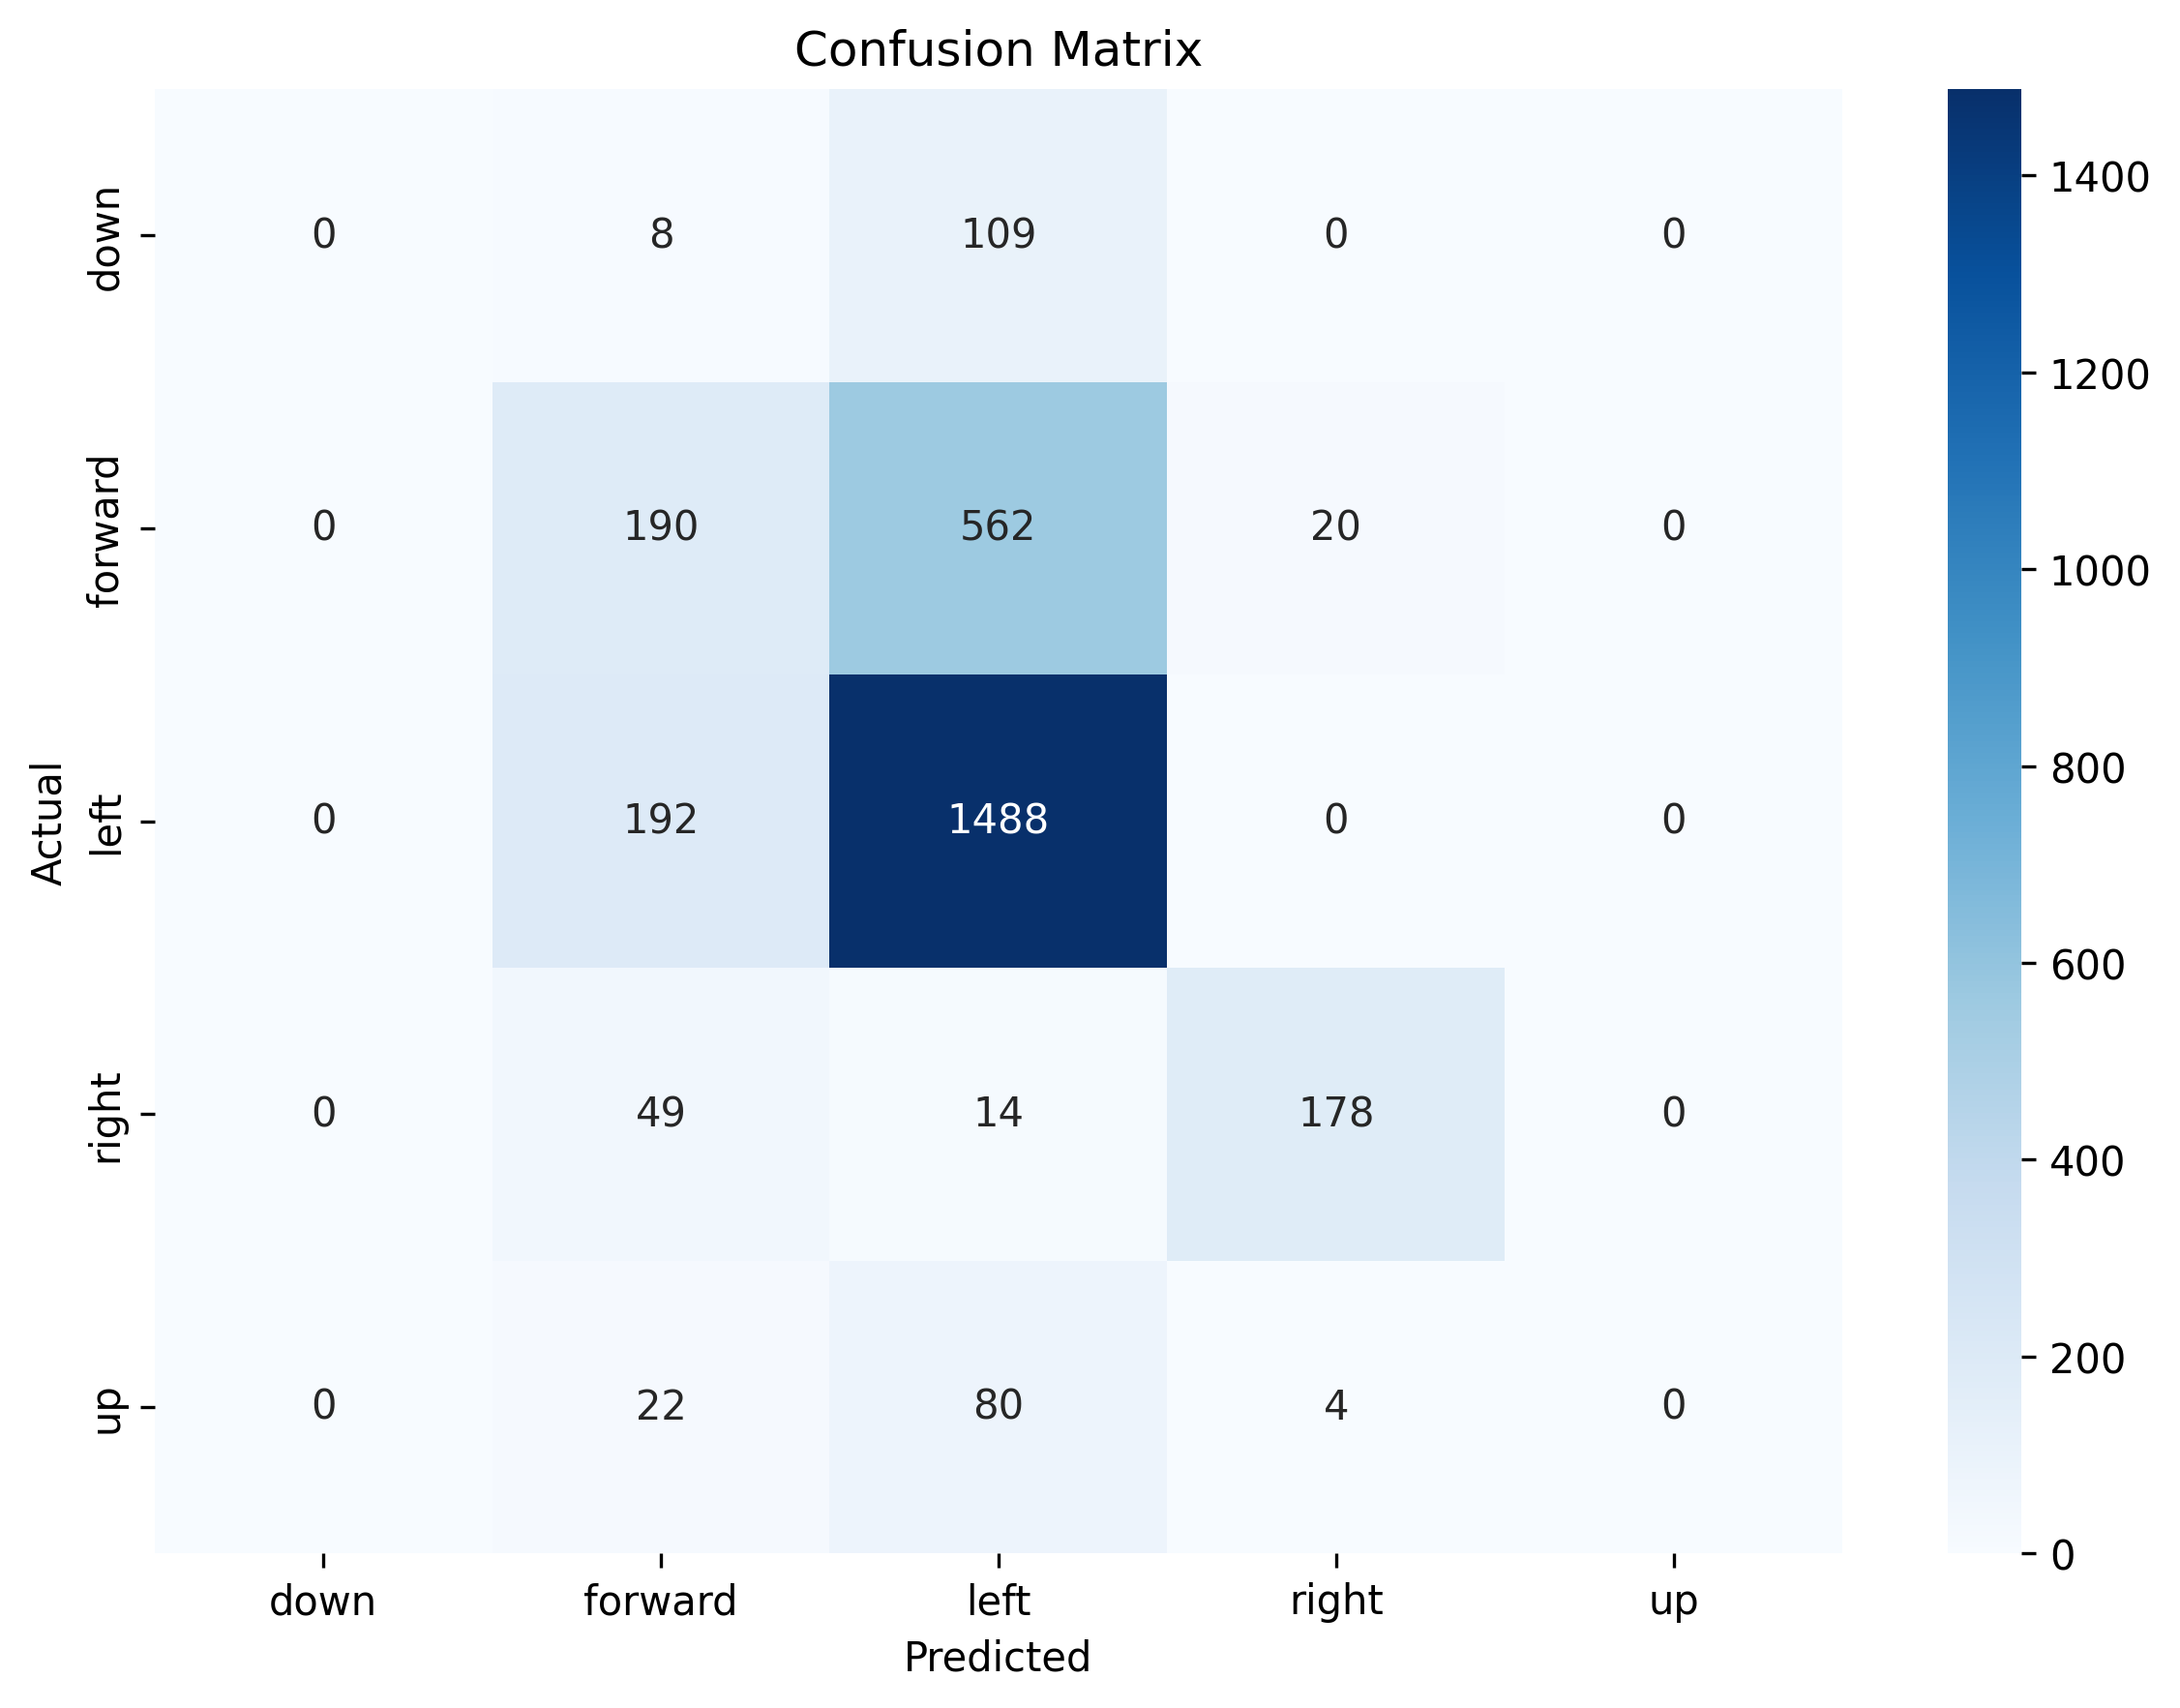
\includegraphics[width=0.85\linewidth]{confusion_matrix.png}
  \caption{Validation confusion matrix for the best MobileNetV2 configuration.}
  \label{fig:cm}
\end{figure}

\subsection{Quantitative Metrics}
Overall validation accuracy is approximately 65\% (exact values depend on split). Per-class precision/recall/F1 can be generated via the provided evaluation routine in \texttt{train\_keras\_head\_pose.py} (classification\_report). We observe higher precision for \emph{left} and \emph{forward}, with reduced recall for \emph{up}/\emph{down}.

\subsection{Model Comparison}
MobileNetV2 outperforms the custom CNN at equal input size due to stronger pretrained features and inverted residual blocks. EfficientNetB0 offers small gains when partially unfrozen but at increased compute. Under frozen-backbone training, MobileNetV2 and EfficientNetB0 are similar.

\section{Discussion}
\paragraph{Why \~65\%?} Factors include (i) dataset size and subject diversity; (ii) class imbalance favoring \emph{left}/\emph{forward}; (iii) coarse labeling near decision boundaries; and (iv) face-detection crop drift on off-axis heads.

\paragraph{Improvements} Balance the dataset and expand subjects; apply stronger augmentation (MixUp/CutMix, blur, coarse dropout); fine-tune by unfreezing top blocks with lower learning rate; use class-weighted or focal loss; consider MobileNetV3/EfficientNetV2-S or 6DRepNet/ HopeNet-style regression. Temporal modeling and multi-modal inputs (depth/IR) can further improve robustness.

\section{Deployment}
We provide an inference utility (ml/inference\_head\_pose.py) that takes RGB images, optionally detects and crops faces via OpenCV cascades, resizes to $160\times160$, and returns class probabilities and top-1 predictions. For multi-person scenes, first run a detector, then route each face to the pose classifier.

\section{Conclusion and Future Work}
Our study demonstrates a deployable HPE pipeline centered on MobileNetV2 achieving \~65--70\% accuracy for coarse pose categorization. Future work includes larger curated datasets (BIWI, 300W-LP, AFLW2000), transformer-based lightweight backbones (DeiT-Ti, MobileViT), semi-supervised pretraining, and multi-task learning with landmarks.

\paragraph{Reproducibility} Training commands and environments are documented in ml/README.md. Random seeds can be fixed in the scripts for determinism where supported.

\bibliographystyle{ieeetr}
\bibliography{refs}

\end{document}

